\section{Lastenheft zur Herstellung des Signalgenerators}
\subsection{Zielbestimmung}
Es soll ein Signalgenerator angefertigt werden. Hierbei ist sich an den Schaltplan und die dort verzeichneten Werte zu halten.
Die verwendeten Bauteile sollen, soweit möglich, SMD-Bauteile sein.\\
Der Umfang des Auftrages umfasst:
\begin{itemize}
\item{das Entwerfen und Herstellen der Platine}
\item{die Beschaffung der Bauteile}
\item{das Bestücken der Platine}
\item{das Programmieren einer Software für den Mikrocontroller des Signalgenerators}
\item{das Erstellen einer Stückliste}
\item{die mechanische und optische Prüfung der Platine}
\end{itemize}

\subsection{Funktionale Anforderungen}

\subsubsection{Platine \& Layout}

Da ein bestimmtes Gehäuse verwendet werden soll, darf die Platine des Signalgenerators nicht größer als
die Innenbemaßung des Gehäuses sein. Eine technische Zeichnung des Gehäuses ist dem Lastenheft beigefügt.\\
Des Weiteren sollte das Layout so angefertigt werden, dass die Mikro-USB Buchse und die SMA-R Buchse gegenüber
an den kurzen Seiten der Platine platziert werden.
Die Platine soll Doublelayer sein und eine Dicke von 1,6mm haben.

\subsubsection{Beschaffen der Bauteile}

Die Bauteile sollen so günstig wie möglich beschafft werden. 

\subsubsection{Bestücken der Platine}

Die Platine ist vollständig zu bestücken und optisch auf Kurzschlüsse zu prüfen.

\subsubsection{Firmware des Mikrocontrollers}

Die Firmware für den Mikrocontroller soll in C geschrieben werden.\\
Zur Ansteuerung des USB-Controllers soll das LUFA Framework verwendet werden.\\
Der Mikrocontroller soll in der Lage sein Daten vom Computer über USB zu empfangen und diese
an die entsprechende Peripherie weiterzugeben. Für die Peripherie sollen ebenfalls die in LUFA enthaltenen Bibliotheken
benutzt werden.\\
Für die USB-Kommunikation soll der Mikrocontroller die VID \VID\ und die PID \PID\ benutzen und sich als Vendorspezifisches HID Gerät anmelden. Für die Kommunikation sollen nur HID-Reports verwendet werden. Der Mikrocontroller soll in der Lage sein bestimmte Daten zurück an den PC zu geben, um Fehleranalyse und Fehlererkennung auf der PC-Seite durchführen zu können.
Auch hierzu ist der Aufbau der zu übertragenden Daten in der Angelegten Protokollspezifikation zu finden.
\pagebreak
\subsection{Anhang}
\subsubsection{Prüfungsvorgabe für die Platinen}
\subsubsection*{Optische Kontrolle}

\begin{flushleft}
	\begin{tabular}{|c||p{10cm}|c|c|}
		\hline
		Nr. & Prüfauftrag & Ja & Nein \\
		\hline
		1 & Sind alle Bauteile bestückt? & & \\
		\hline
		2 & Sind alle Bauteile fachgerecht gelötet? & & \\
		\hline
		3 & Sind IC-Beine miteinander verbunden, die nicht miteinander verbunden sein dürfen? & & \\
		\hline
		4 & der Fädeldraht zum aktivieren der USB-Schnittstelle des Mikrocontrollers ist eingelötet & & \\
		\hline
		5 & Der Lötjumper zum aktivieren des LT1615 ist gesetzt & & \\
		\hline
	\end{tabular}
\end{flushleft}


\subsubsection*{Elektrische Kontrolle}
Die folgenden Messungen sind mit einem Digitalmultimeter durchzuführen. Sollte einer der Widerstände \underline{nicht} den Anforderungen entsprechen, so darf die Platine unter keinen Umständen einer Funktionskontrolle unterzogen werden.
\begin{flushleft}
	\begin{tabular}{|c||p{10cm}|c|c|p{2cm}|}
		\hline
		Nr. & Prüfauftrag & Ja & Nein & Wert\\
		\hline
		1 & Messen des Widerstandes zwischen $V_{cc}$ und GND. Ist der Wert größer als 900$\Omega$? & & &\\
		\hline
		2 & Messen des Widerstandes zwischen $USB_{D+}$ und GND. Ist der Wert größer als 500k$\Omega$? & & & \\
		\hline
		3 & Messen des Widerstandes zwischen $USB_{D-}$ und GND. Ist der Wert größer als 500k$\Omega$? & & & \\
		\hline
		4 & Messen des Widerstandes zwischen +12V und GND. Ist der Wert größer als 50k$\Omega$? & & & \\
		\hline
		5 & Messen des Widerstandes zwischen -12V und GND. Ist der Wert größer als 10k$\Omega$? &&& \\
		\hline
		6 & Messen des Widerstandes zwischen +3.3V und GND. Ist der Wert größer als 2k$\Omega$? &&& \\
		\hline
		7 & Messen des Widerstandes zwischen -3.3V und GND. Ist der Wert größer als 2k$\Omega$? &&& \\
		\hline
		8 & Messen Sie die Stromaufnahme des Signalgenerators. Ist der Strom kleiner gleich 100mA? &&& \\
		\hline
	\end{tabular}
\end{flushleft}

\subsubsection{Gehäuseplan}
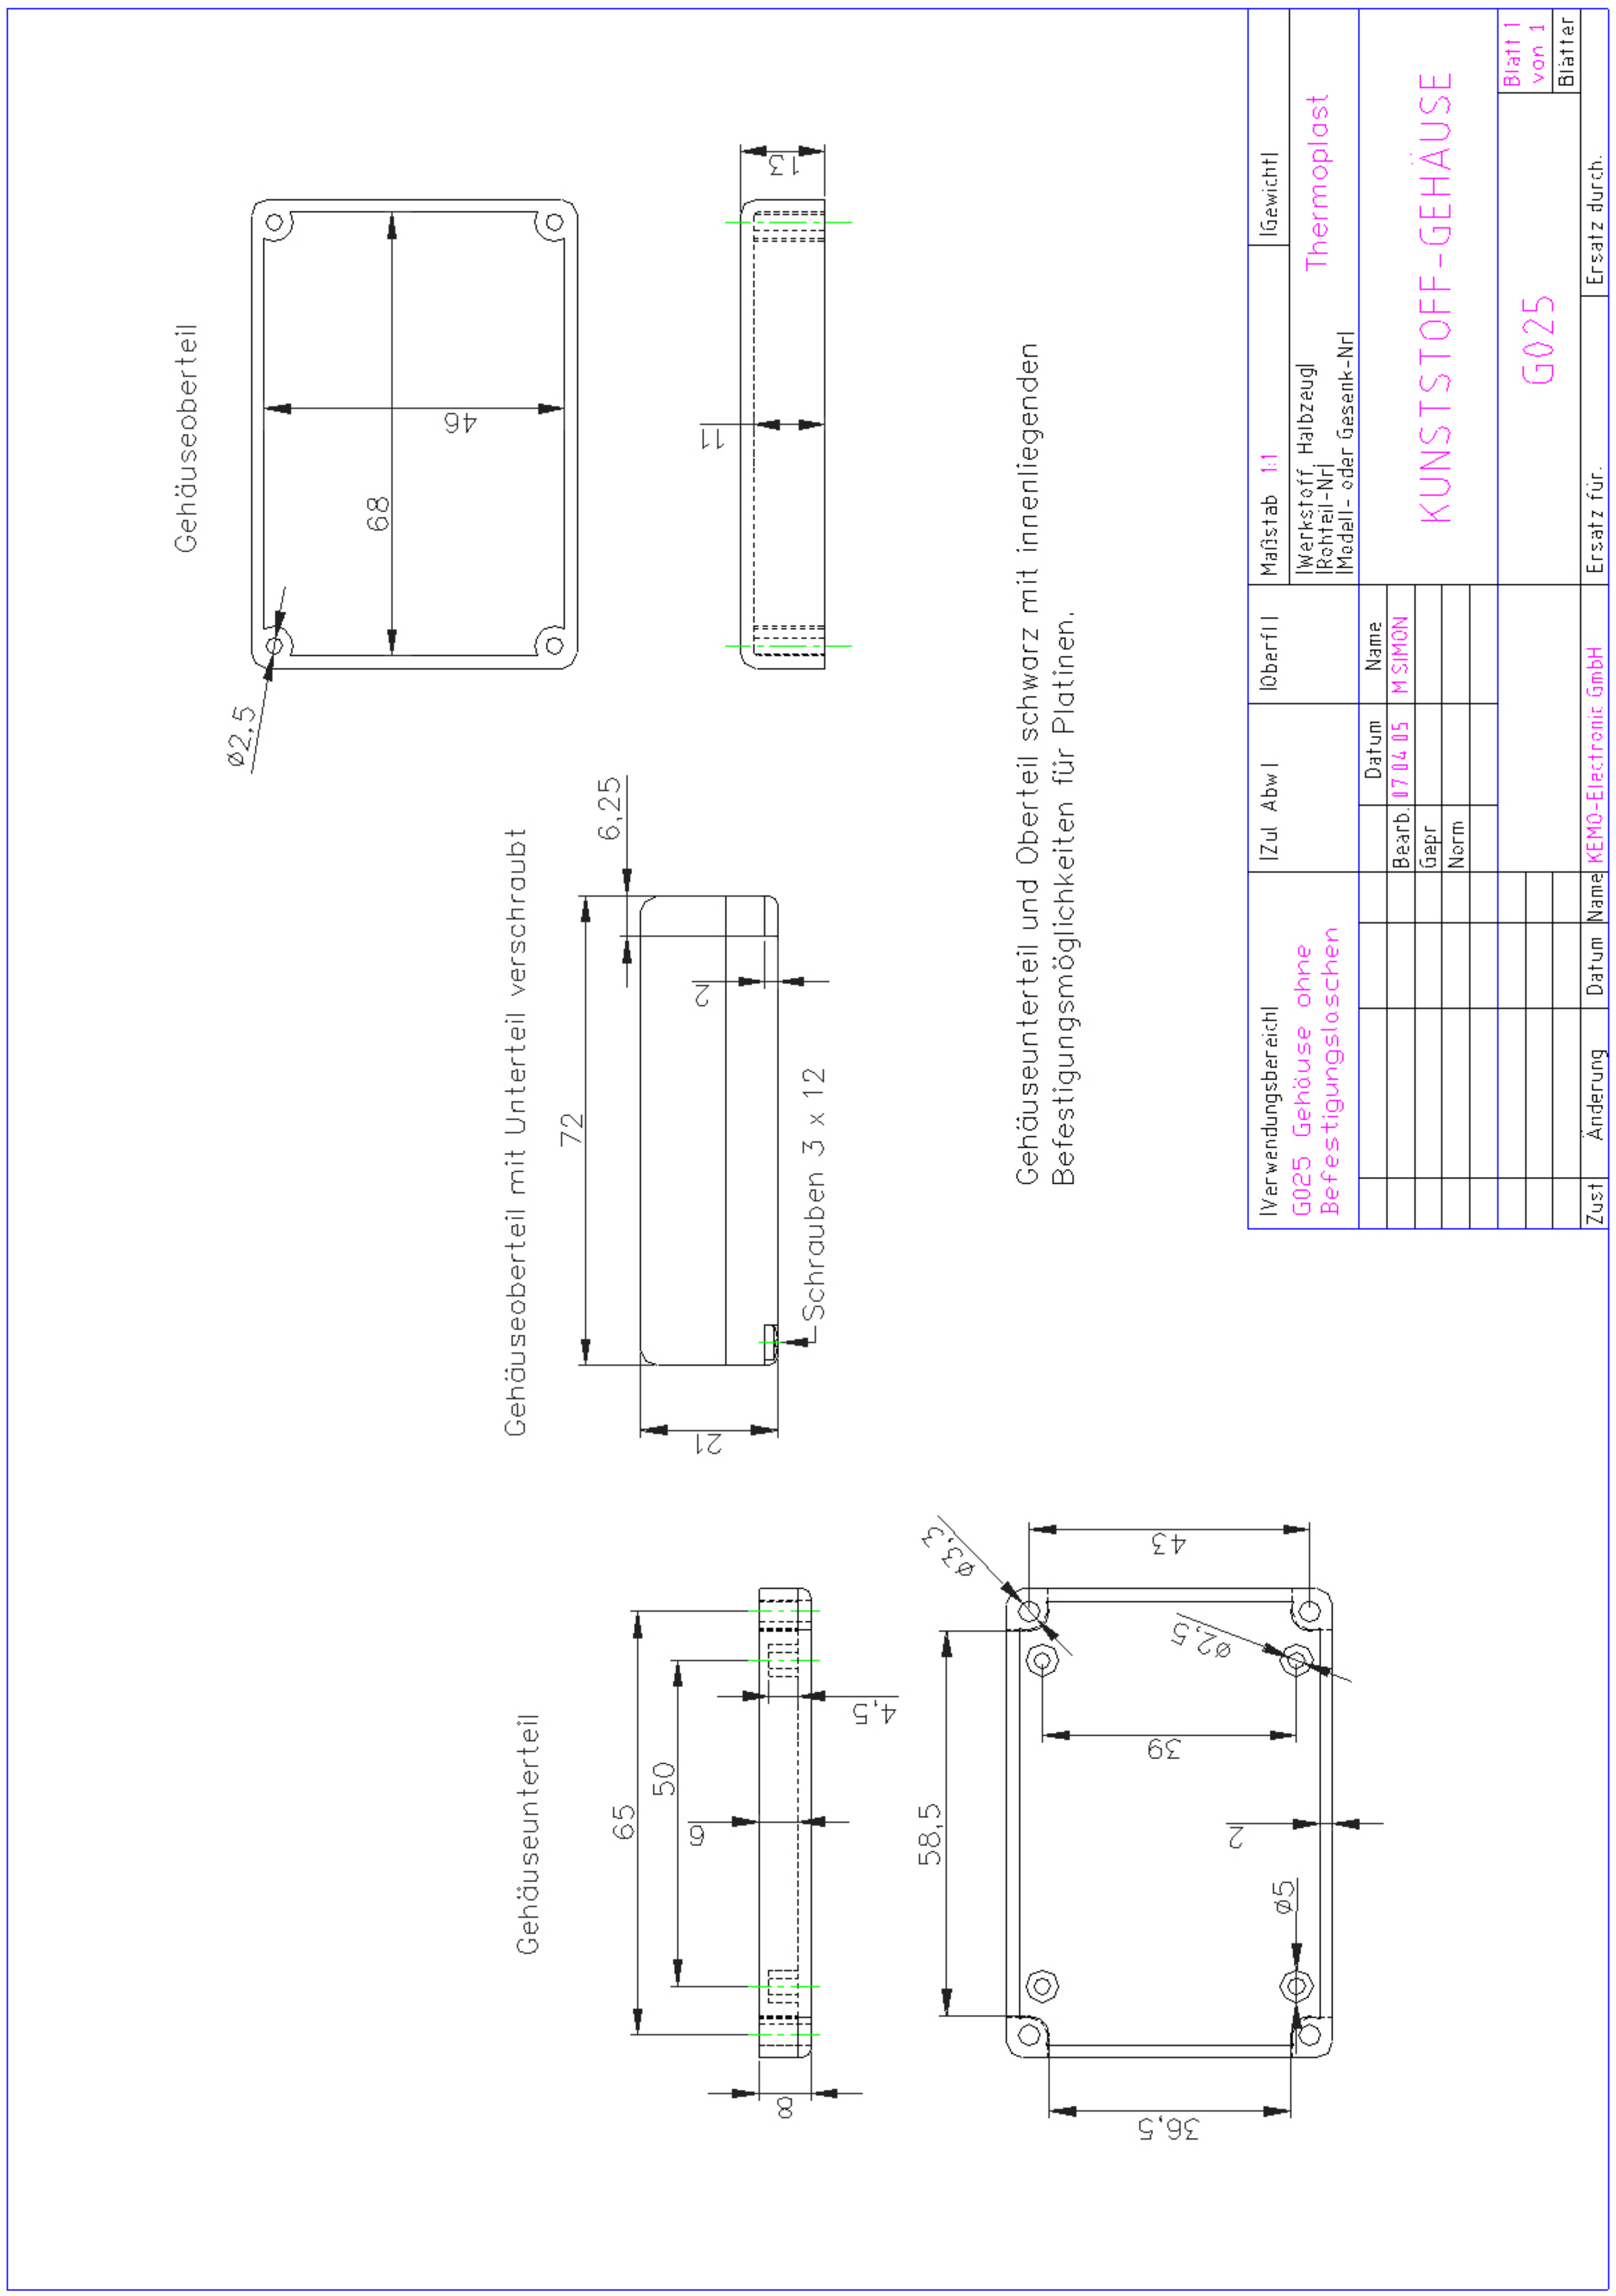
\includegraphics[scale=1]{./img/Gehauseplan.png}